\documentclass[12pt,a4paper]{article}

\input{../../preamble_files/packages}
\input{../../preamble_files/scriptr}
\input{../../preamble_files/siunits}
\input{../../preamble_files/vectors}
\input{../../preamble_files/figures}
\input{../../preamble_files/references}
\input{../../preamble_files/empheq}

\pagestyle{fancy}
\lhead{Richard Whitehill}
\chead{PHYS 631 -- HW F}
\rhead{02/10/22}
\cfoot{\thepage \hspace{1pt} of \pageref{LastPage}}

\newcommand{\prob}[2]{\textbf{#1)} #2}

\setlength{\parskip}{\baselineskip}
\setlength{\parindent}{0pt}

\begin{document}

\prob{2.22}{Find the potential a distance $s$ from an infinitely long straight wire that carries a uniform line charge $\lambda$. Compute the gradient of your potential, and check that it yields the correct field.}

\bef
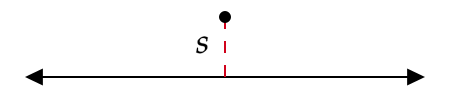
\includegraphics[scale=0.5]{fig1.png}
\eef

We see that
\begin{align*}
V = -\int \va*{E} \vdot \dd{\va*{\ell}} = -\frac{\lambda}{2\pi\epsilon_0}\int_{s_0}^{s} \frac{1}{s'} \dd{s}
\end{align*}
\begin{eqbox}
V = \frac{\lambda}{2\pi\epsilon_0}\ln(\frac{s_0}{s})
\end{eqbox}
where $s_0$ is an arbitrary reference point not on the wire or at infinity (e.g. $s_0 = 1$ in units of length). We can check this result as follows:
\begin{align*}
\va*{E} = -\grad{V} = -\pdv{V}{s}\shat = \frac{\lambda}{2\pi\epsilon_0}\pdv{s}\ln(\frac{s}{s_0}) =  \frac{1}{2\pi\epsilon_0}\frac{\lambda}{s}
\end{align*}

\prob{2.23}{For the charge configuration of Prob. 2.15, find the potential at the center, using infinity as your reference point.}

\bef
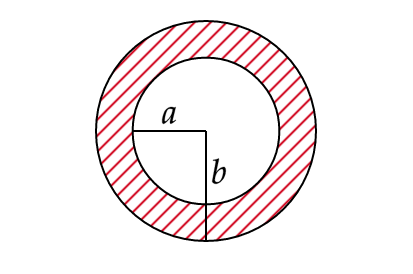
\includegraphics[scale=0.5]{fig2.png}
\eef

Notice that the electric field, using spheres as our Gaussian surfaces, is
\begin{align*}
E = \frac{k}{\epsilon_0}\begin{cases}
0, & r < a \\
\frac{r-a}{r^2}, & a < r < b \\
\frac{b-a}{r^2}, & r > b
\end{cases}
\end{align*}

Then, the potential at the center, using infinity as our reference, is
\begin{align*}
V &= -\int_{0}^{\infty} E \dd{r} = -\frac{k}{\epsilon_0}\qty[ \int_{0}^{a} 0\dd{r} + \int_{a}^{b} \frac{r-a}{r^2} \dd{r} + \int_{b}^{\infty} \frac{b-a}{r^2} \dd{r}] \\
&= -\qty[\ln(b) + \frac{a}{b} - \ln(a) - 1 + \frac{b-a}{b}]
\end{align*}
\begin{eqbox}
V = -\frac{k}{\epsilon_0}\ln(\frac{b}{a})
\end{eqbox}

\end{document}
